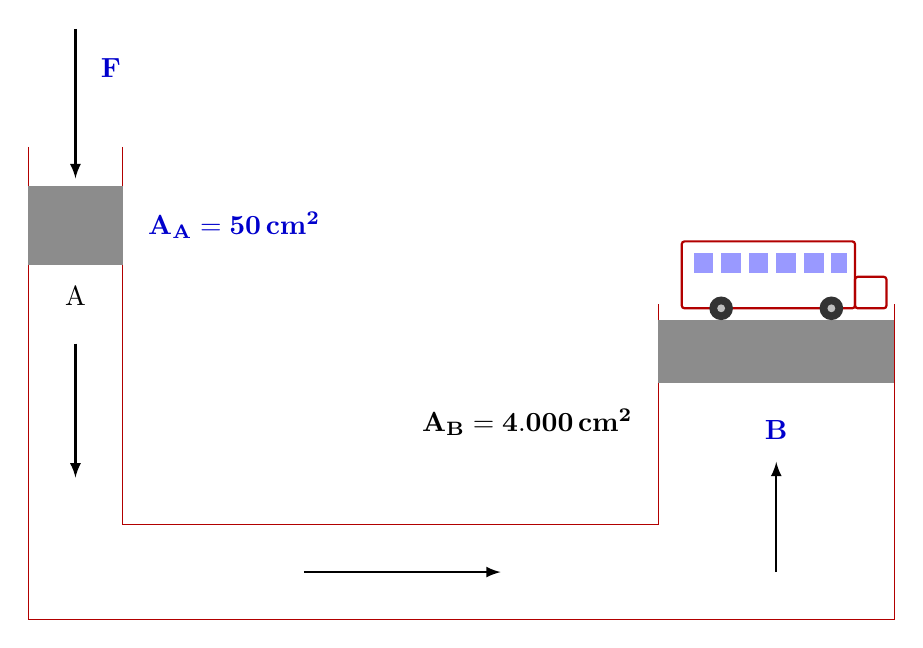
\begin{tikzpicture}[>=latex]

    % Definición de colores para igualar la imagen
    \colorlet{tubered}{red!70!black}
    \colorlet{piston}{gray!90}
    \colorlet{labelblue}{blue!80!black}

    % 1. Trazado del tubo en U (líneas rojas)
    % Borde exterior
    \draw[ tubered] (0, 6) -- (0, 0) -- (11, 0) -- (11, 4);
    % Borde interior
    \draw[ tubered] (1.2, 6) -- (1.2, 1.2) -- (8, 1.2) -- (8, 4);

    % 2. Pistón A (Izquierda, más pequeño)
    \fill[piston] (0, 4.5) rectangle (1.2, 5.5);
    \node[] at (0.6, 4.1) {A};

    % 3. Pistón B (Derecha, más grande)
    \fill[piston] (8, 3.0) rectangle (11, 3.8);

    % 4. Dibujo simplificado del autobús sobre el Pistón B
    \begin{scope}[shift={(8.3, 3.8)}]
        % Carrocería principal
        \draw[thick, tubered, rounded corners=1pt] (0, 0.15) rectangle (2.2, 1.0);
        % Capó/Frente
        \draw[thick, tubered, rounded corners=1pt] (2.2, 0.15) rectangle (2.6, 0.55);
        
        % Ruedas
        \fill[black!80] (0.5, 0.15) circle (0.15);
        \fill[black!80] (1.9, 0.15) circle (0.15);
        \fill[gray!50] (0.5, 0.15) circle (0.05); % Centro de la rueda
        \fill[gray!50] (1.9, 0.15) circle (0.05); % Centro de la rueda
        
        % Ventanas de pasajeros
        \foreach \x in {0.15, 0.5, 0.85, 1.2, 1.55} {
            \fill[blue!40] (\x, 0.6) rectangle (\x+0.25, 0.85);
        }
        % Ventana del conductor
        \fill[blue!40] (1.9, 0.6) rectangle (2.1, 0.85);
    \end{scope}

    % 5. Flechas y Etiquetas

    % Fuerza F entrante (Arriba izquierda)
    \draw[->, thick] (0.6, 7.5) -- (0.6, 5.6);
    \node[labelblue, right] at (0.8, 7.0) {\textbf{F}};

    % Área A
    \node[labelblue, right] at (1.4, 5.0) {$\mathbf{A_A = 50 \, cm^2}$};

    % Flecha de flujo descendente (Tubo izquierdo)
    \draw[->, thick] (0.6, 3.5) -- (0.6, 1.8);

    % Flecha de flujo horizontal (Tubo inferior)
    \draw[->, thick] (3.5, 0.6) -- (6.0, 0.6);

    % Flecha de flujo ascendente (Tubo derecho)
    \draw[->, thick] (9.5, 0.6) -- (9.5, 2.0);
    \node[labelblue] at (9.5, 2.4) {\textbf{B}};

    % Área B
    \node[ left] at (7.8, 2.5) {$\mathbf{A_B = 4.000 \, cm^2}$};

\end{tikzpicture}
